\chapter{Background Knowledge}

\section{A brief overview of \gls{dms}}
In the 1980s, printers, scanners, and household computers started to gain popularity.
Organizations start to take actions on managing their information records and assets seriously.
At that time, Document Image Processing (DIP) systems are the only available software to satisfy their needs.
DIP is the electronic version of filing cabinet where documents need to be scanned, indexed, and store in the system \cite{1_adam_2008}.
DIP can also analyse figures, texts, and handwriting \cite{akram2010document} using various image processing techniques.
\begin{wrapfigure}{l}{0.5\textwidth}
	\centering
	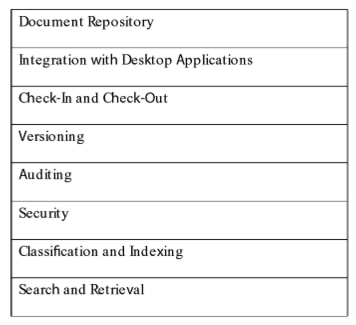
\includegraphics[scale=0.7]{res/bg-knowledge/edms-components.png}
	\caption{Components of EDMS \citefigure{1_adam_2008}}
	\label{fig:edms-components}
\end{wrapfigure}
Later on in the 1990s, Electronics Document Management System (EDMS) is developed targeting large enterprises with high volume of documents.
It is the improved version of DIP with workflow functionality.
Workflow functionality enables organizations to passed around scanned document throughout the organization to designated employee.
EDMS also has its own document repository allowing documents to be indexed and tracked using version control.
There are various sub-types of EDMS such as Electronic Record Management Systems (ERMS) deals mainly with record keeping.
Enterprise Content Management (ECM), suites of applications, deals with document and record management.
Nowadays, EDMS acronym is shortened to DMS.
Figure \ref{fig:edms-components} shows a basic components of DMS.
Most DMS applications have these components implemented within.
\begin{description}
	\item[Document Repository] \hfill \\
	A place where indexed documents are stored.
	Typically on a hard disk of a network server.
	\item[Integration with desktop applications] \hfill \\
	Allowing user to save documents straight to application when document is created.
	It is usually a 3rd party add-on embedded in popular office applications such as Microsoft Office.
	\item[Check-in and check-out] \hfill \\
	This feature controls who is allowed to make changes or to read documents.
	Basically, it is a user permission control system.
	\item[Versioning] \hfill \\
	Keeping track of changes by assigning a version number to a document.
	The number is incremented after the document passes major revisions.
	User can access the previous versions of the document.
	\item[Auditing] \hfill \\
	Track who changes document, when, and where.
	Only authorized user can read these information.
	\item[Security] \hfill \\
	Controls how documents should be stored in the server to prevent hackers from attacking the system.
	\item[Classification and indexing] \hfill \\
	Metadata and tags provide more information to documents.
	It helps to search and retrieve documents easier.
	\item[Search and Retrieval] \hfill \\
	Allow user to retrieve documents according to keywords.
	Keywords can be a metadata or contents within a document.
	A system may offer advance search criteria by looking for individual fields and combine with other fields using basic logical operations (AND, OR, NOT). 
\end{description}

\section{What is Metadata}
Metadata literally means \enquote{data about data} \cite[p.~1]{baca_2008}.
Brackett \cite[p.149]{brackett_2000} defined metadata in terms of organization as \enquote{Any data about organization's resource}.
There is no clear definition on what metadata is because this term is used differently in different communities.
For librarians, it refers to information in the library catalog that help users to find the right book in the library.
For search engines, it means descriptions of web page's contents and keywords used to rank relevant websites.
For others, it may refer to a descriptive information of resources in human readable format.
Whatever metadata refers to, they share the following similar usage.
\begin{enumerate}
	\item To identify resources.
	\item To distinguish or bundle similar resources.
	\item To find resources based on search criteria.
\end{enumerate}
There are 3 types of metadata \cite{hodge_2001}.
\begin{description}
	\item[Descriptive metadata] give a description of resources for discovery and identification.
	\item[Structural metadata] describes how component's objects are organized.
	\item[Administrative metadata] indicates information about how resource suppose to be managed.
\end{description}

\begin{figure}[h]
	\centering
	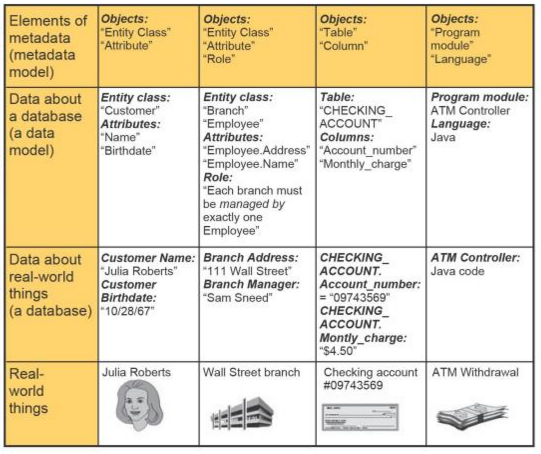
\includegraphics[scale=0.8]{res/bg-knowledge/data-and-metadata}
	\caption{data and metadata \citefigure{hay_2006}}
	\label{fig:data-metadata}
\end{figure}
Figure \ref{fig:data-metadata} provides simple model examples of how metadata represents real-world things.
Each column shows different examples.
The third row is a descriptive metadata.
Julia Robert is the customer's name and 10/28/67 is her birthdate.
These 2 metadata refer to only this \enquote{Julia Roberts} 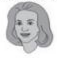
\includegraphics[scale=0.3]{res/bg-knowledge/metadata-julia} and not any other Julia Roberts. 
Same with a second example, A branch in \enquote{111 Wall Street} with a branch manager \enquote{Sam Sneed} refer to this 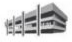
\includegraphics[scale=0.3]{res/bg-knowledge/metadata-wallstreet} branch only.
The next row up is a structured metadata.
It shows a higher abstraction concept to describe general real-world things.
Julia Roberts can be generalized as a \enquote{Customer} entity with \enquote{Name} and \enquote{Birthdate} as its attributes.
A checking account in the third example can be generalized as a table called \enquote{CHECKING\_ACCOUNT} with \enquote{Account\_number} and \enquote{Monthly\_charge} as its columns.

\section{NoSQL}
\gls{nosql} is a database that does not use \gls{sql}.
It refers to any database that does not follow the traditional \gls{rdbms} model.
\gls{sql} was designed to be a query language for relational databases, and they are usually table-based.
Records are stored in rows and columns represent fields.
On the other hand, \gls{nosql} allow to define fields while creating a record.
Nested values are common in \gls{nosql} databases because \gls{nosql} is aggregate oriented.
Hashes and arrays and objects, and then nest more objects and arrays and hashes within those.

The main characteristic separating \gls{nosql} databases from relational \gls{sql} databases is that they do not use query languages derived from \gls{sql}. 
The following list shows common features of \gls{nosql} \cite[p.~12 - 16]{nosql-for-dummies}.
\begin{description}
	\item[Schema agnostic] \hfill \\
	\gls{nosql} databases doesn't require schema to be defined explicitly.
	Any type of records can be stored without having to know how databases store them internally.
	\item[Nonrelational] \hfill \\
	A relational database needs relations to describe how tables relate to each other.
	Unlike \gls{rdbms}, \gls{nosql} databases don't have any relation concept.
	They don't store how each record relate to each other but rather graph database with key-value pairs.
	\item[Highly distributable] \hfill \\
	A single server may not be able to handle all data requests in time.
	Instead of dedicating database on the single server, many servers needed to process queries in parallel.
	Storing data across multiple servers in relational databases is a challenging task.
	\gls{nosql} databases can handle distributed queries as long as connected machines are fast enough to talk to each other.
\end{description}

There are many \gls{nosql} storage types available to model the content.
For example, \enquote{Column-oriented database} stores data as columns instead of rows in \gls{rdbms}.
\enquote{Graph store} represents data as nodes and relationships as edges in a graph.
This report will focus on \enquote{Document Store} storage type.
\gls{nosql} databases with \enquote{Document Store} storage type organized data as a hierarchical model with parent-child relationships.
The topmost node in Figure \ref{arch-node} called a root node.
This node is required as a starting point for a record and the model must have only one root node.
\begin{figure}[h]
	\centering
	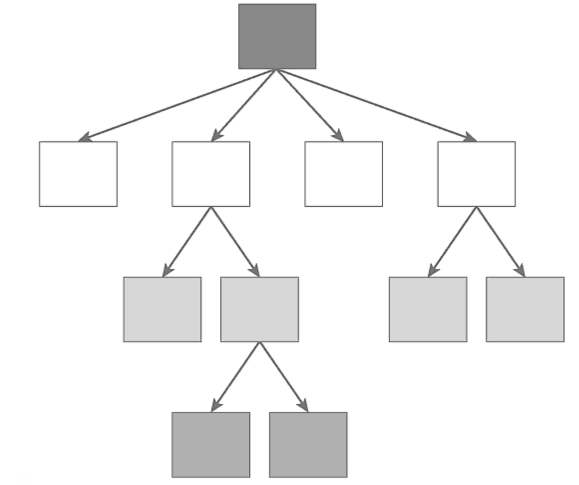
\includegraphics[scale=0.48]{res/bg-knowledge/nosql-hierarchical}
	\caption{The hierarchical organized into a set of parent-child nodes \citefigure{nosql-for-mere-mortals}}
	\label{arch-node}
\end{figure}
Directed Edges connecting between two nodes represents relations.
A node where an arrow points called a parent node.
A node where an arrow is pointed called a child node.
The parent node can many child nodes and each child node can have many parent nodes.

For example, a simple customer's receipt with orders and billing addresses from figure \ref{nosql-aggregate-uml} can be modelled to hierarchical parent-child structure in figure \ref{nosql-aggregate-uml-realized}. 
Each node is an object in itself.
\gls{nosql} database can locate any node within the graph according to any specific queries.
\begin{figure}[h]
	\centering
	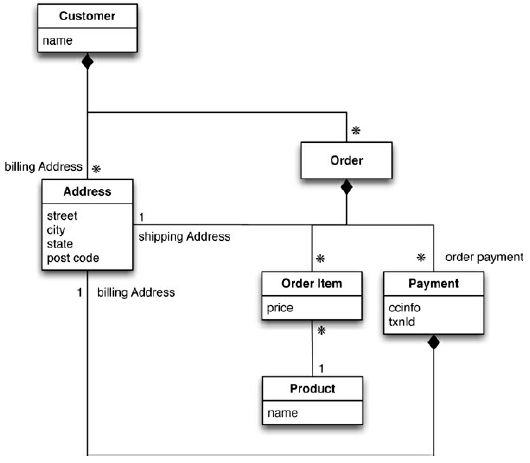
\includegraphics[scale=0.55]{res/bg-knowledge/nosql-nosql-agregate-uml}
	\caption{An aggregate data model in UML notation \citefigure{sadalage_fowler_2013}}
	\label{nosql-aggregate-uml}
\end{figure}
\begin{figure}[h]
	\centering
	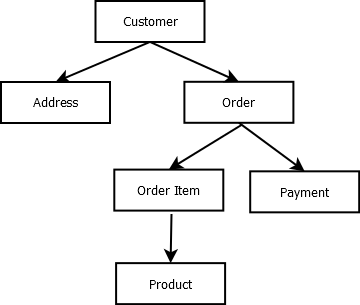
\includegraphics[scale=0.5]{res/bg-knowledge/nosql-uml-realized}
	\caption{A hierarchical structure representation from figure \ref{nosql-aggregate-uml}}
	\label{nosql-aggregate-uml-realized}
\end{figure}

Most databases use \gls{xml}, \gls{json}, \gls{bson}, or \gls{yaml} to manipulate data.
Client have to use REST API provided by the database to query the data.
\gls{rest} is a network-based software architectural style of the World Wide Web \cite{doglio, masse_2012}.
It takes care interactions between client and server.
Client program communicates with the database using \gls{http} through exposed \glspl{api}.

Table \ref{tbl:doctype-storage-feature} summarize key features of \gls{nosql} database with \enquote{Document Store} storage type.
\begin{table}[h]
	\centering
	\begin{tabular}{l c}
		\hline
		Feature                             &      Document Store \\
		\hline
		Table-like schema support (columns) &      No \\
		Complete update/fetch               &      Yes \\
		Partial update/fetch                &      Yes \\
		Query/Filter on	value               &      Yes \\
		Aggregates across rows              &      No \\
		Relationships between entities      &      No \\
		Cross-entity view support           &      Yes \\
		Batch fetch                         &      Yes \\
		Batch update                        &      Yes \\
		\hline
	\end{tabular}
	\caption{Sumarization of available features for \enquote{Document Store} storage type \citefigure{vaish_2013} \cite{vaish_2013}}
	\label{tbl:doctype-storage-feature}
\end{table}

\glsreset{bpmn}
\section{\gls{bpmn}}
\gls{bpmn} is a graphical notation that depicts the steps in business process \cite{bpmn_omg}.
% What
The goal is to represent business processes using standard graphical notation.
% Who
\gls{bpmn} targets business users and process implementers who need a standard model to communicate their business process.
% Why
Business users create, manage, and monitor processes while process implementers turn processes into a physical implementation. 
\gls{bpmn} doesn't focus on why, when, and how a process is performed.
But rather what processes, which are the steps to achieve that process, and who should do them.
With \gls{bpmn}, organizations can understand, improve, and control their business processes.

% Provide example

% elements and diagrams
Table \ref{tbl:sum-bpmn-symbol} summarizes \gls{bpmn} symbols that appear in this report along with its short description.
Please refer to http://www.omg.org/cgi-bin/doc?formal/11-01-03.pdf (page 28 - 41) for more details on all available \gls{bpmn} symbols and its detailed descriptions.
%TODO UPDATE NEW SYMBOLS AS IT APPEARS IN THIS REPORT
\begin{table}
	\centering
	\caption{Summary of \gls{bpmn} symbols}
	\label{tbl:sum-bpmn-symbol}
\begin{tabular}{m{0.2\textwidth} m{0.5\textwidth} m{0.2\textwidth}}
	\hline
	Element & Description & Notation \\
	\hline
	Start Event & Indicates where a process begins & \bpmnfig{\bpmnSymRepo{start-event-none}} \\
	End Event & Indicates where a process will end & \bpmnfig{\bpmnSymRepo{end-event-none}}
\end{tabular}
\end{table}